\documentclass{report}

\usepackage[utf8]{inputenc}
\usepackage[T1]{fontenc}
\usepackage[francais]{babel}
\usepackage{graphicx}
\usepackage{url}
\usepackage{hyperref}
\hypersetup{colorlinks= true,urlcolor= black}

\title{Projet de Technologie du Web 2013}
\author{HOSSAINY Said Samim (\url{mailto:said.hossainy@etudiant.univ-lille1.fr}) \\ 
DIAGNE Salla (\url{mailto:salla.diagne@etudiant.univ-lille1.fr})}
\date{URL de test : \url{http://webtp.fil.univ-lille1.fr/~diagne/projetTW/sources}}

\begin{document}

\maketitle

\section*{Introduction}
\og City Finder \fg est un service de cartographie centrée qui permet de rechercher une ou plusieurs communes françaises situées sur une carte. À l'issue d'une recherche, des marqueurs symbolisant chaque commune résultat (s'il y en a) sont positionnés sur la carte. Le service permet également d'afficher des détails complets pour chaque commune résultat et, si on le désire, de l'ajouter à nos favoris.
\section*{Informations générales}
Le travail réalisé est en corrélation avec ce qui a été demandé, toutes les instructions concernant ce projet ont été suivies et respectées.
\subsubsection*{Descriptif nécessaire à l'utilisation du site}
\begin{itemize}
\item une barre de recherche située en haut à droite de la page d'accueil appelée barre de recherche rapide, permet de rechercher une commune par son nom.
\\
\end{itemize}
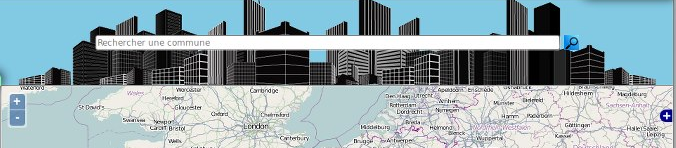
\includegraphics[width=12.1cm]{rr.png}
\\
\begin{itemize}
\item une 2\ieme \ zone, située à gauche de l'écran dans l'onglet recherche, est réservée à une exploration plus complète avec 6 critères de recherche.
\\
\end{itemize}
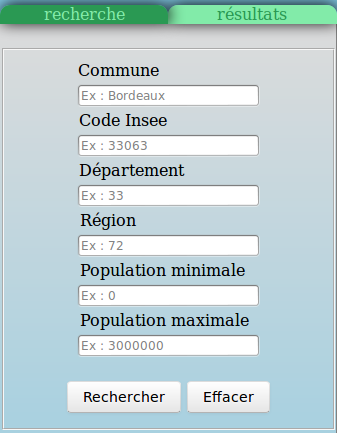
\includegraphics[height=6cm]{ra.png}
\\
\begin{itemize}
\item la 3\ieme \ zone de la page d'accueil est occupée par la carte, sur laquelle sont affichés les marqueurs de chaque commune figurant dans les résultats d'une recherche. Le zoom de la carte est adaptée aux marqueurs qui y sont positionnés (elle a été configurée pour afficher tous les marqueurs de la carte, peu importe leurs positions).
Un clic sur un résultat dans la liste redirigera l'utilisateur vers une page détails qui listera tout ce qu'il faut savoir sur la commune en question à côté d'une carte zoomée.
\\
\end{itemize}
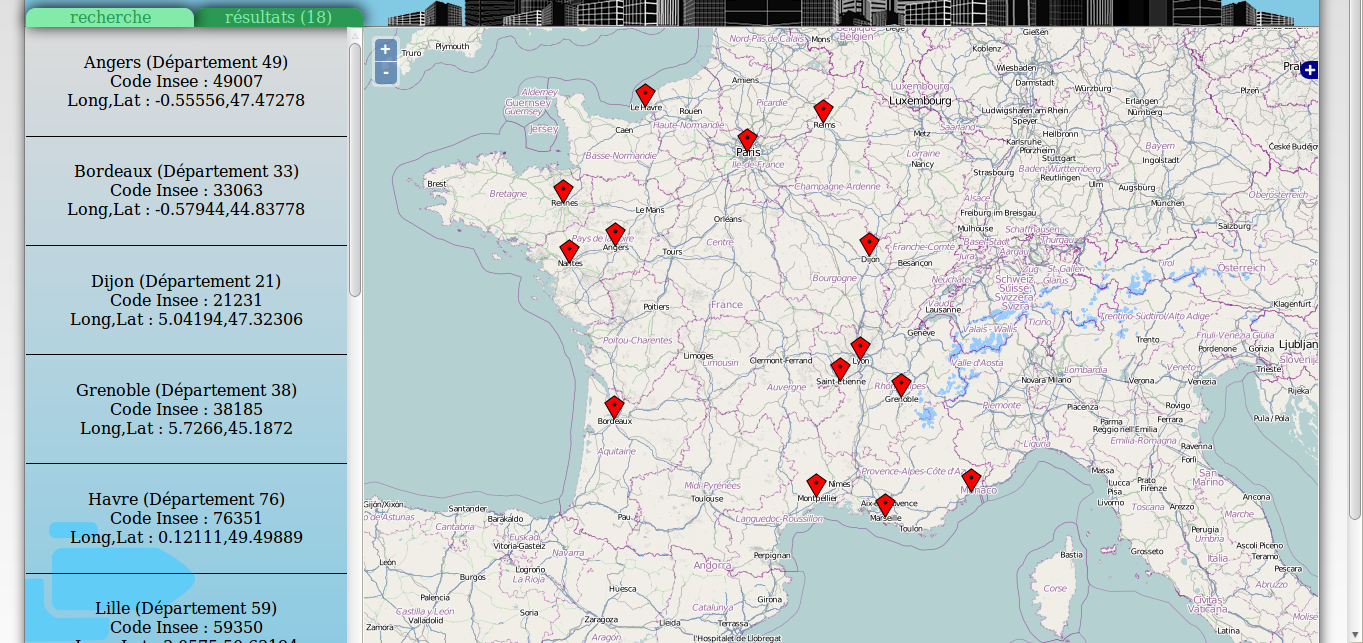
\includegraphics[width=12.1cm]{main.png}
\\
\textit{Exemple d'une recherche concernant les communes qui ont une population supérieure ou égale à 150000 habitants (les grandes villes).}
\\
\begin{itemize}
\item une barre de favoris située en haut à droite de la page permet, comme son nom laisse deviner, d'afficher les communes favorites de l'utilisateur. Un clic sur une de ces communes redirigera l'utilisateur vers une page détails de la commune. L'ajout d'une commune aux favoris se fait depuis cette page détails.
\\
\end{itemize}
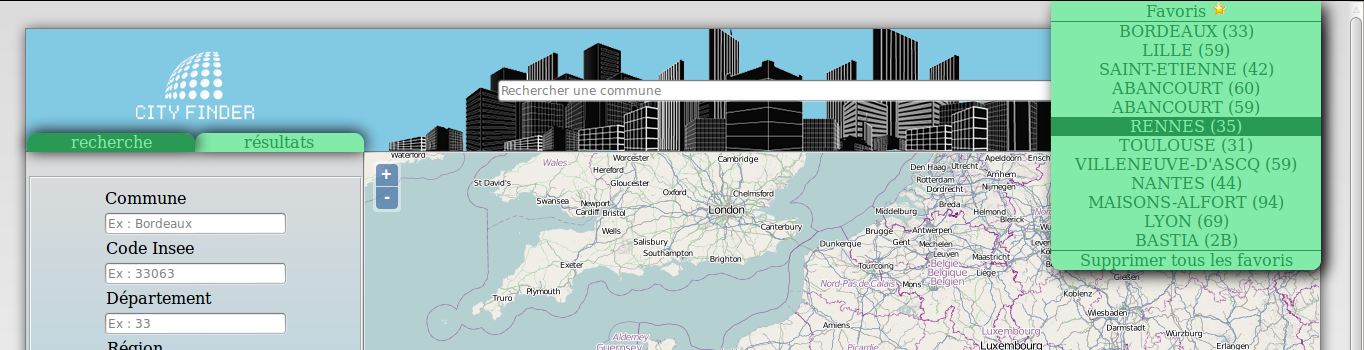
\includegraphics[width=12.1cm]{favoris.png}
\\
\textit{L'apparence de la barre de favoris avec quelques communes ajoutées (curseur positionné sur Rennes).}
\\\\
\subsubsection*{Principaux choix d'implémentation}
\begin{itemize}
\item le site en lui-même est présenté sous la forme d'une grande table avec deux lignes de deux cellules chacune, et parfois des sous-cellules dans quelques-unes de ces cellules.
\item les onglets recherche et résultats sont gérés en Javascript grâce à une méthode \lq\lq\ afficher-cacher \rq\rq,caractéristique classique des onglets. Ainsi,l'onglet recherche est sélectionné par défaut (écritures vertes claires sur fond vert foncé), et l'onglet résultats est caché (écritures vertes foncées sur fond vert clair).
\item le formulaire de recherche rapide permet de rechercher une commune en fonction de son nom, le champ est évidemment requis puisqu'il est unique et donc le formulaire n'est pas validé tant que ce champ n'est pas rempli. Une fois le champ rempli et la validation effectuée, le contenu du champ est récupéré en PHP par une méthode POST et est transformé en majuscules si nécessaire; puis la base de données est interrogée par une requête SQL et les résultats sont affichés, triés par pertinence, dans l'onglet résultat qui sera sélectionné depuis la validation du formulaire. Un résultat comporte le nom de la commune, son département, son code insee et ses coordonnées. Il est possible de rechercher plusieurs communes à la fois, en les séparant par un ou des espaces.
\item le formulaire de recherche avancée, qui comporte 6 champs, permet d'affiner sa recherche, avec notamment la possibilité de renseigner le code insee, la population minimale, etc. Un message d'alerte apparaît si aucun champ n'est rempli. Si au moins un champ est rempli, le ou les champs remplis sont récupérés en POST et sont traitées par un tableau progressif (voir fichier \lq rechercheAvancee.php \rq) et les résultats sont affichés après interrogation de la base de données. Une pagination est mise en place si la recherche a donné plus de 15 résultats. Comme mentionné plus haut, un clic sur un résultat d'un des deux modes de recherche conduit à une page qui présentera les détails de la commune à côté d'une carte zoomée sur cette commune.
\item la page détails affiche des informations sur la commune sélectionnée dans les résultats. En plus de ceux qui figuraient dans l'onglet résultats, l'utilisateur aura ainsi des renseignements supplémentaires sur la commune, comme par exemple son nombre d'habitants, la région à laquelle elle appartient, ou encore ses chefs-lieu. Depuis cette page de détails, l'utilisateur peut ajouter la commune à ses favoris si elle n'y figure pas, la retirer si elle y figure, et/ou retourner à la page d'accueil.
\item la liste des communes favorites peut être consultée en survolant le menu déroulant de la barre des favoris (en haut à droite de la page détails). L'utilisateur peut cliquer sur une commune pour accéder à sa page détails, et éventuellement la retirer des favoris de là-bas, ou tout simplement supprimer l'ensemble de ses favoris en cliquant sur le bouton \lq\lq\ Supprimer tous les favoris \rq\rq. L'ajout et le retrait d'une commune des favoris est géré par un système de cookies.
\end{itemize}
\section*{Liste des fichiers du projet}
\begin{description}
\item[affichageFavoris.php :] permet d'afficher les communes favorites de l'utilisateur, qui a la possibilité de les visualiser en consultant la barre des favoris. Si le tableau de cookies n'existe pas (s'il n'a pas mis de commune à ses favoris), le message \lq\lq\ Vous n'avez pas de commune favorite pour le moment \rq\rq s'affiche; sinon, chaque valeur du tableau est affiché (nom de la commune + département) et un bouton \lq\lq\ Supprimer tous les favoris est créé \rq\rq.
\item[Commune.class.php :] classe représentant une commune. Cette classe possède 8 attributs (nom, code département, code commune, code région, coordonnées(2), tncc et population) et un constructeur à 8 paramètres, représentant les attributs de la classe. La méthode getCharniere renvoie la charnière de la commune en fonction de son tncc, les méthodes afficheResultat et afficheDetails permettent d'afficher la commune respectivement dans l'onglet résultat et dans la page détails, et espacement gère l'espace entre le nom de la commune et sa charnière.
\item[connect.php :] ce fichier permet de se connecter dans la base de données du projet. Il crée un nouvel objet PDO qui représentera la connexion à projetTW. Le fichier doit être inclus dans chaque fichier qui interroge la base.
\item[details.css :] c'est la feuille de style de la page détails. Des commentaires plus précis sont présents dans le fichier lui-même.
\item[details.php :] ce fichier représente la page détails d'une commune. La page elle-même est présentée en deux parties : la partie gauche qui affiche les détails et permet de gérer la commune par rapport à ses favoris et/ou de retourner à la page précédente, et la partie droite qui affichera la carte zoomée sur la commune. Le titre de la page est le nom de la commune.
\item[detailsCommune.php :] ce fichier est chargé d'afficher les détails concernant une commune depuis sa page de détails. Il crée un objet Commune avec les paramètres nécessaires et invoque la méthode afficheDetails.
\item[index.css :] c'est le fichier principal de la \lq\lq\ forme \rq\rq\ du site. Il permet de styliser correctement la page d'acceuil. Des commentaires plus précis sont présents dans le fichier lui-même.
\item[index.js :] c'est le seul fichier Javascript du projet, mais il n'en est pas moins fondamental. En effet, ce fichier gère entièrement la carte (affichage et centrage sur la France, ajout des marqueurs des communes-résultats et zoom sur la commune dans la page détails); il permet aussi le jonglage entre les onglets recherche et résultats et par conséquent la pagination, d'afficher le nombre de résultats d'une recherche, de gérer les favoris et le message du bloc selon l'ajout ou le retrait, le message d'alerte si aucun champ du formulaire de la recherche avancée n'est rempli, et enfin la suppression de tous les favoris.
\item[index.php :] c'est le fichier central du site, celui qui est affiché au lancement du site. Il contient entre autres tout le descriptif nécessaire à l'utilisation du site.
\item[pagination.php :] c'est le fichier qui permet de mettre en place la pagination des résultats. Il contient une fonction pagination qui a pour paramètre la page courante et le nombre de pages et un appel à cette fonction en fonction de la page courante qui est passée dans l'url à l'affichage des résultats et du nombre de pages qui est une variable session définie après la requête SQL.
\item[rechercheAvancee.php :] ce fichier se charge principalement de récupérer le contenu des champs remplis dans le formulaire, d'interroger la base de données, d'afficher les 15 premiers résultats tout en sauvegardant tout le tableau des résultats dans une variable de session qui sera utiliser pour afficher les 15 correspondant à la page que l'on veut visiter. Il stocke aussi l'url courant dans une autre variable de session (utile quand on veut revenir à la page précédente depuis la page détails).
\item[rechercheRapide.php :] c'est le fichier qui traite la recherche rapide. À la différence du nombre de champs traités, il a exactement le même fonctionnement que le fichier \lq rechercheAvancee.php\rq.
\item[titreDetails.php :] il permet de changer le titre du document en fonction de la commune en question depuis la page détails. Il utilise une fonction getArticle qui renvoie l'article adéquat en fonction du tncc, interroge la base en fonction du code insee de la commune passée dans l'url, récupère le tncc, le nom, et code département de la commune et à fortiori change le titre de la page.
\end{description}
\end{document}